\chapter{System Implementation}

\section{Module Description}

\begin{itemize}

\item \textbf{Frontend Module:}
The frontend is a React and TypeScript single-page application built with Vite. It contains the public landing page, customer authentication screens, sample restaurant and menu browsing, cart and checkout demonstrations, profile screens, and role-specific demonstration portals. Restaurant and menu content is currently bundled as sample data. The frontend sends registration and login requests to the authentication API and sends chatbot messages to the assistant service.

\item \textbf{Backend Module:}
The backend is a Node.js and Express API written in TypeScript. It provides routes for authentication, roles, restaurant and profile data, menu items, image uploads, orders, dashboards, and chatbot assistance. Zod schemas validate request payloads. CORS, Helmet, Morgan, and Dotenv are included for API configuration, headers, request logging, and environment-variable loading.

\item \textbf{Database Module:}
The backend is connected to MySQL through a connection pool whose settings are read from environment variables. The eight-table schema was initialized, and the restaurant API returns records from MySQL. The schema defines users, restaurants, rider and restaurant profiles, categories, menu items, uploaded images, and orders. Authentication can use a file-backed fallback when database operations fail. The customer storefront still uses bundled data, and its cart and checkout screens do not create persistent orders.

\item \textbf{Chatbot Module:}
The chatbot calls the backend assistant endpoint and uses Gemini with a server-side API key. The configured primary model is \texttt{gemini-3.8-flash}; transient HTTP 429 and 5xx errors trigger one retry with exponential backoff and jitter. If primary generation fails, the backend tries \texttt{gemini-3.6-flash} once, then the chatbot route retains its local rule-based fallback. Conversation history is passed to the model, and a Gemini-generated recipe response was verified during testing. The assistant provides guidance; it does not access live order data, provide personalized food recommendations, or place orders on the user's behalf.

\end{itemize}

\section{Current Application Screens}

The following screenshots were captured from the current frontend. After the confirmation screen, the delivery screen displays zoomable OpenStreetMap tiles centered on Bhubaneswar. Its approximate city-center marker and scripted order timeline are demonstrations, not live rider GPS tracking. The screens should not be interpreted as evidence of live payment processing, persistent orders, or production authorization.

\subsection{Landing Page and Customer Home}

\begin{figure}[H]
    \centering
    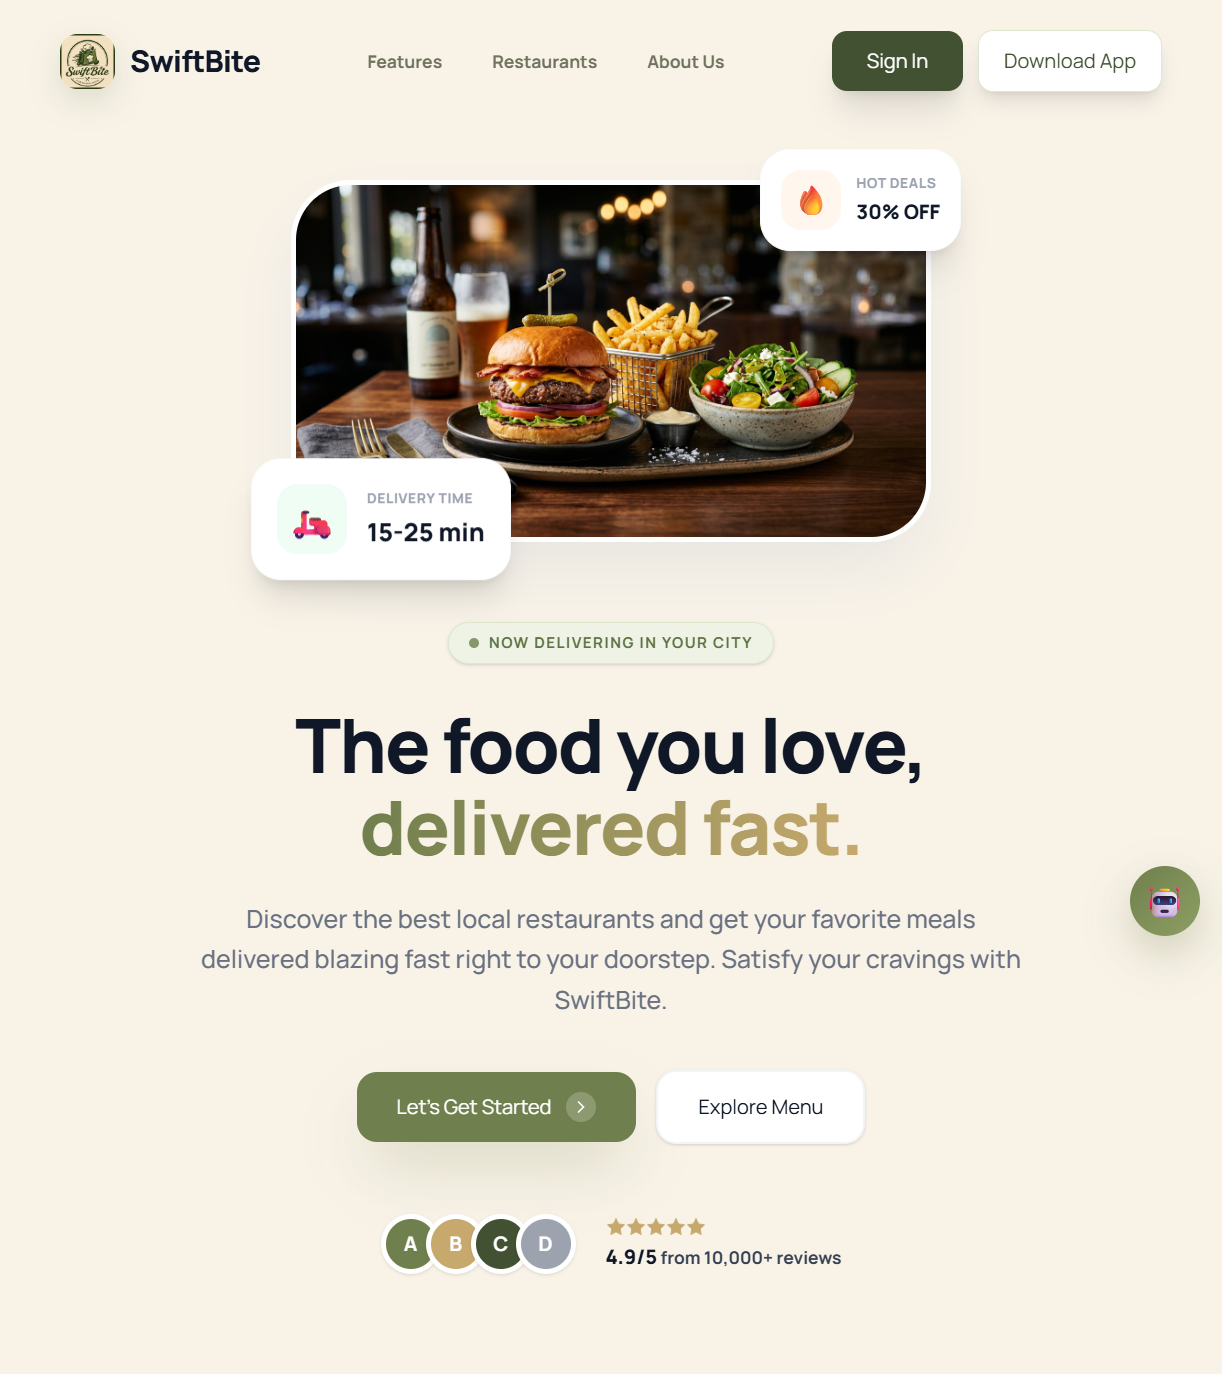
\includegraphics[width=0.9\textwidth,height=0.5\textheight,keepaspectratio]{Chapters/landing_page.png}
    \caption{Current SwiftBite landing page}
    \label{fig:landing_page}
\end{figure}

\begin{figure}[H]
    \centering
    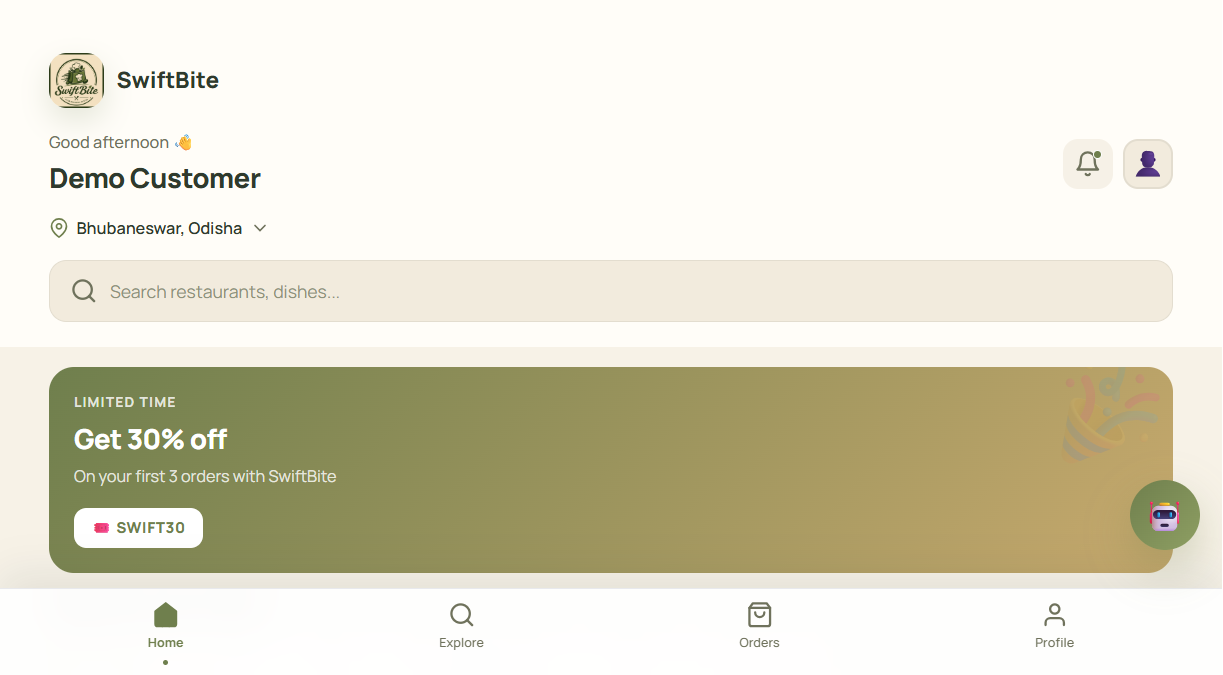
\includegraphics[width=0.9\textwidth,height=0.35\textheight,keepaspectratio]{Chapters/customer_home.png}
    \caption{Customer home screen showing the current promotion and food categories}
    \label{fig:customer_home}
\end{figure}

\subsection{Registration and Password Confirmation}

\begin{figure}[H]
    \centering
    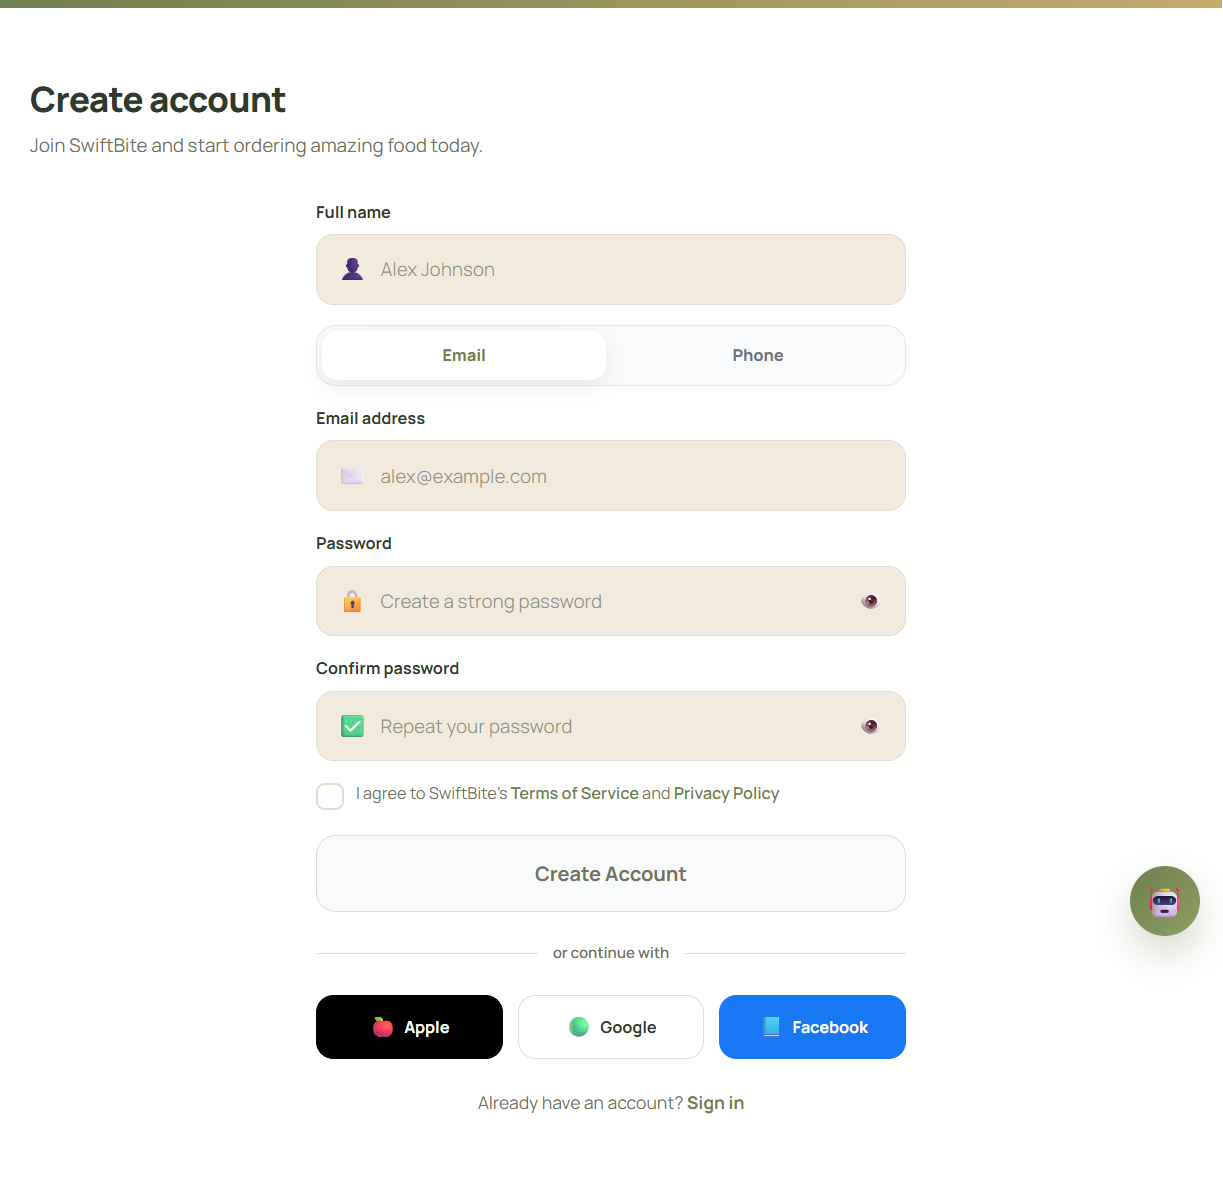
\includegraphics[width=0.72\textwidth,height=0.4\textheight,keepaspectratio]{Chapters/register.png}
    \caption{Current sign-up form, including the required confirm-password field}
    \label{fig:register_current}
\end{figure}

\begin{figure}[H]
    \centering
    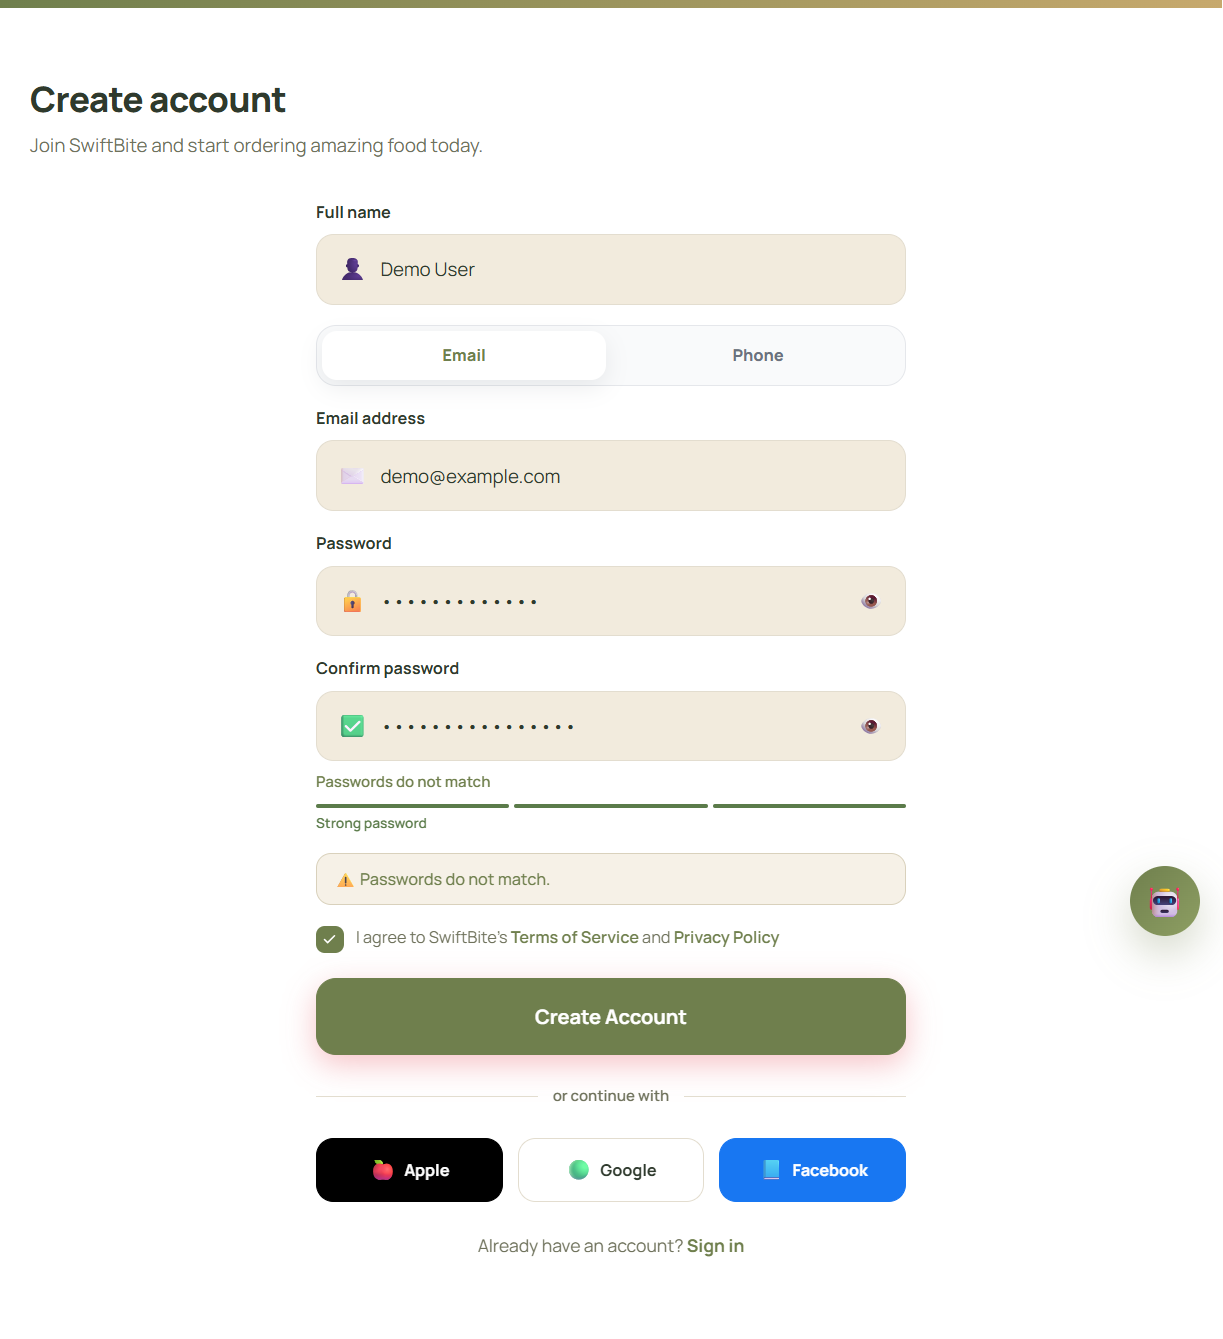
\includegraphics[width=0.72\textwidth,height=0.4\textheight,keepaspectratio]{Chapters/validation_error.png}
    \caption{Current sign-up validation when the password fields do not match}
    \label{fig:password_validation}
\end{figure}

\subsection{Restaurant Menu and Checkout}

\begin{figure}[H]
    \centering
    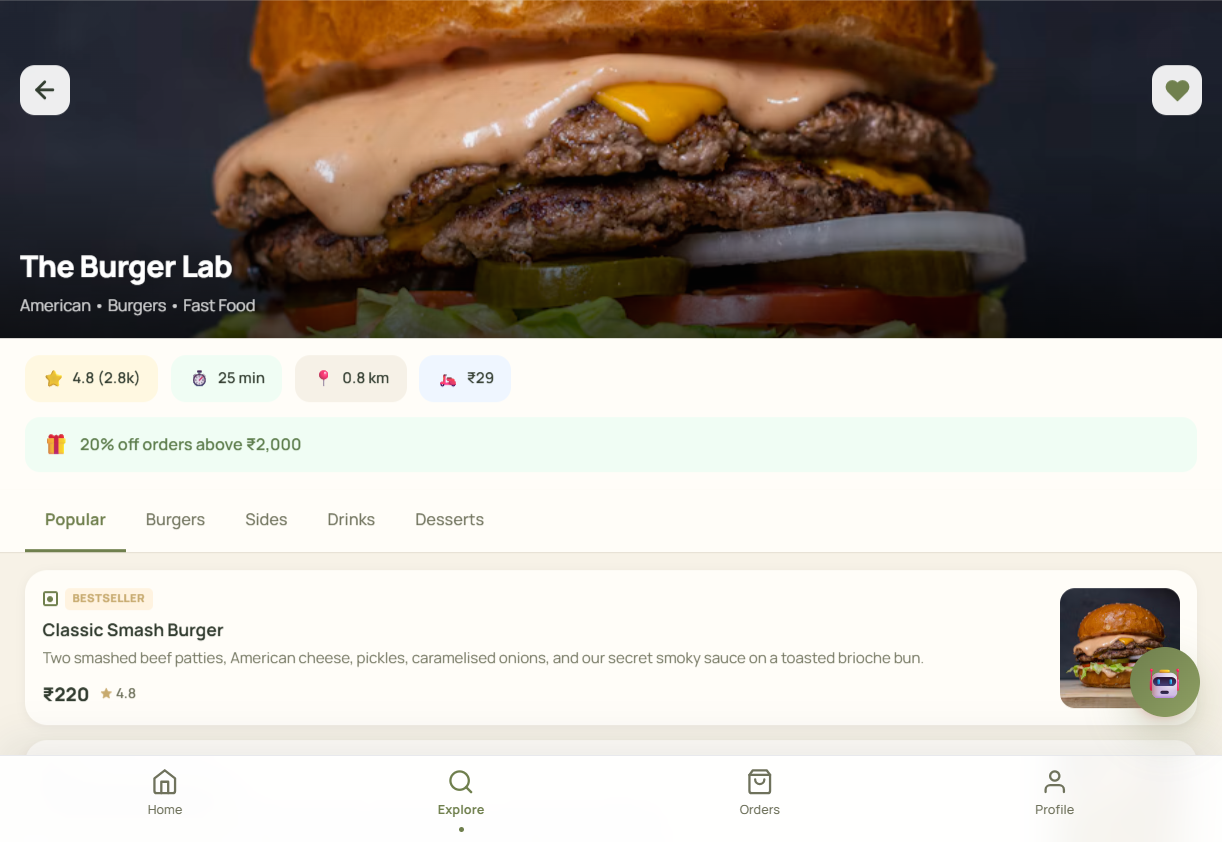
\includegraphics[width=0.9\textwidth,height=0.58\textheight,keepaspectratio]{Chapters/menu_list.png}
    \caption{Restaurant detail and sample menu}
    \label{fig:menu_current}
\end{figure}

\begin{figure}[H]
    \centering
    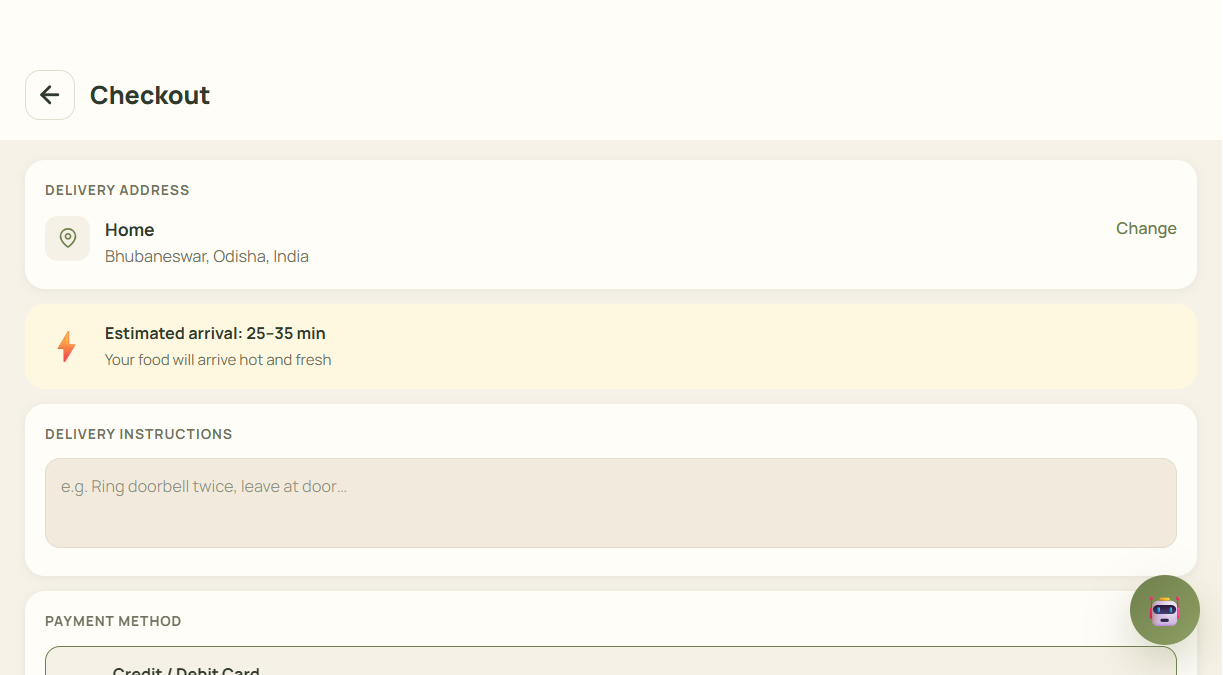
\includegraphics[width=0.9\textwidth,height=0.45\textheight,keepaspectratio]{Chapters/checkout.png}
    \caption{Checkout demonstration with delivery and payment-selection options}
    \label{fig:checkout_current}
\end{figure}

\subsection{Order Status, Chatbot, and Portal Switching}

\begin{figure}[H]
    \centering
    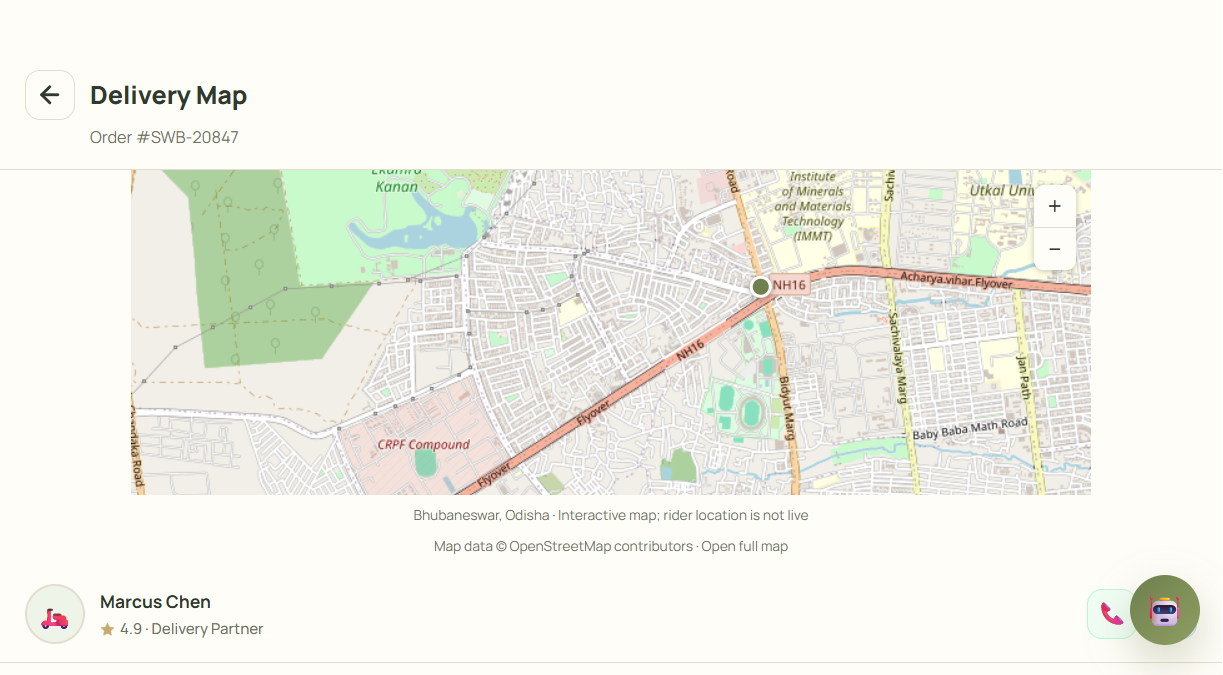
\includegraphics[width=0.9\textwidth,height=0.9\textheight,keepaspectratio]{Chapters/order_tracking_bhubaneswar_app.png}
    \caption{SwiftBite delivery screen with zoomable OpenStreetMap tiles centered on Bhubaneswar; rider location is not live}
    \label{fig:tracking_current}
\end{figure}

\begin{figure}[H]
    \centering
    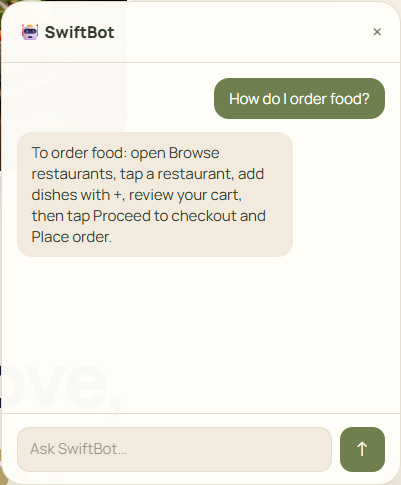
\includegraphics[width=0.9\textwidth,height=0.4\textheight,keepaspectratio]{Chapters/chatbot_test.png}
    \caption{Local rule-based chatbot fallback response to an app-guidance question}
    \label{fig:chatbot_current}
\end{figure}

\begin{figure}[H]
    \centering
    \vspace*{2cm}
    \hspace*{3.5cm}
    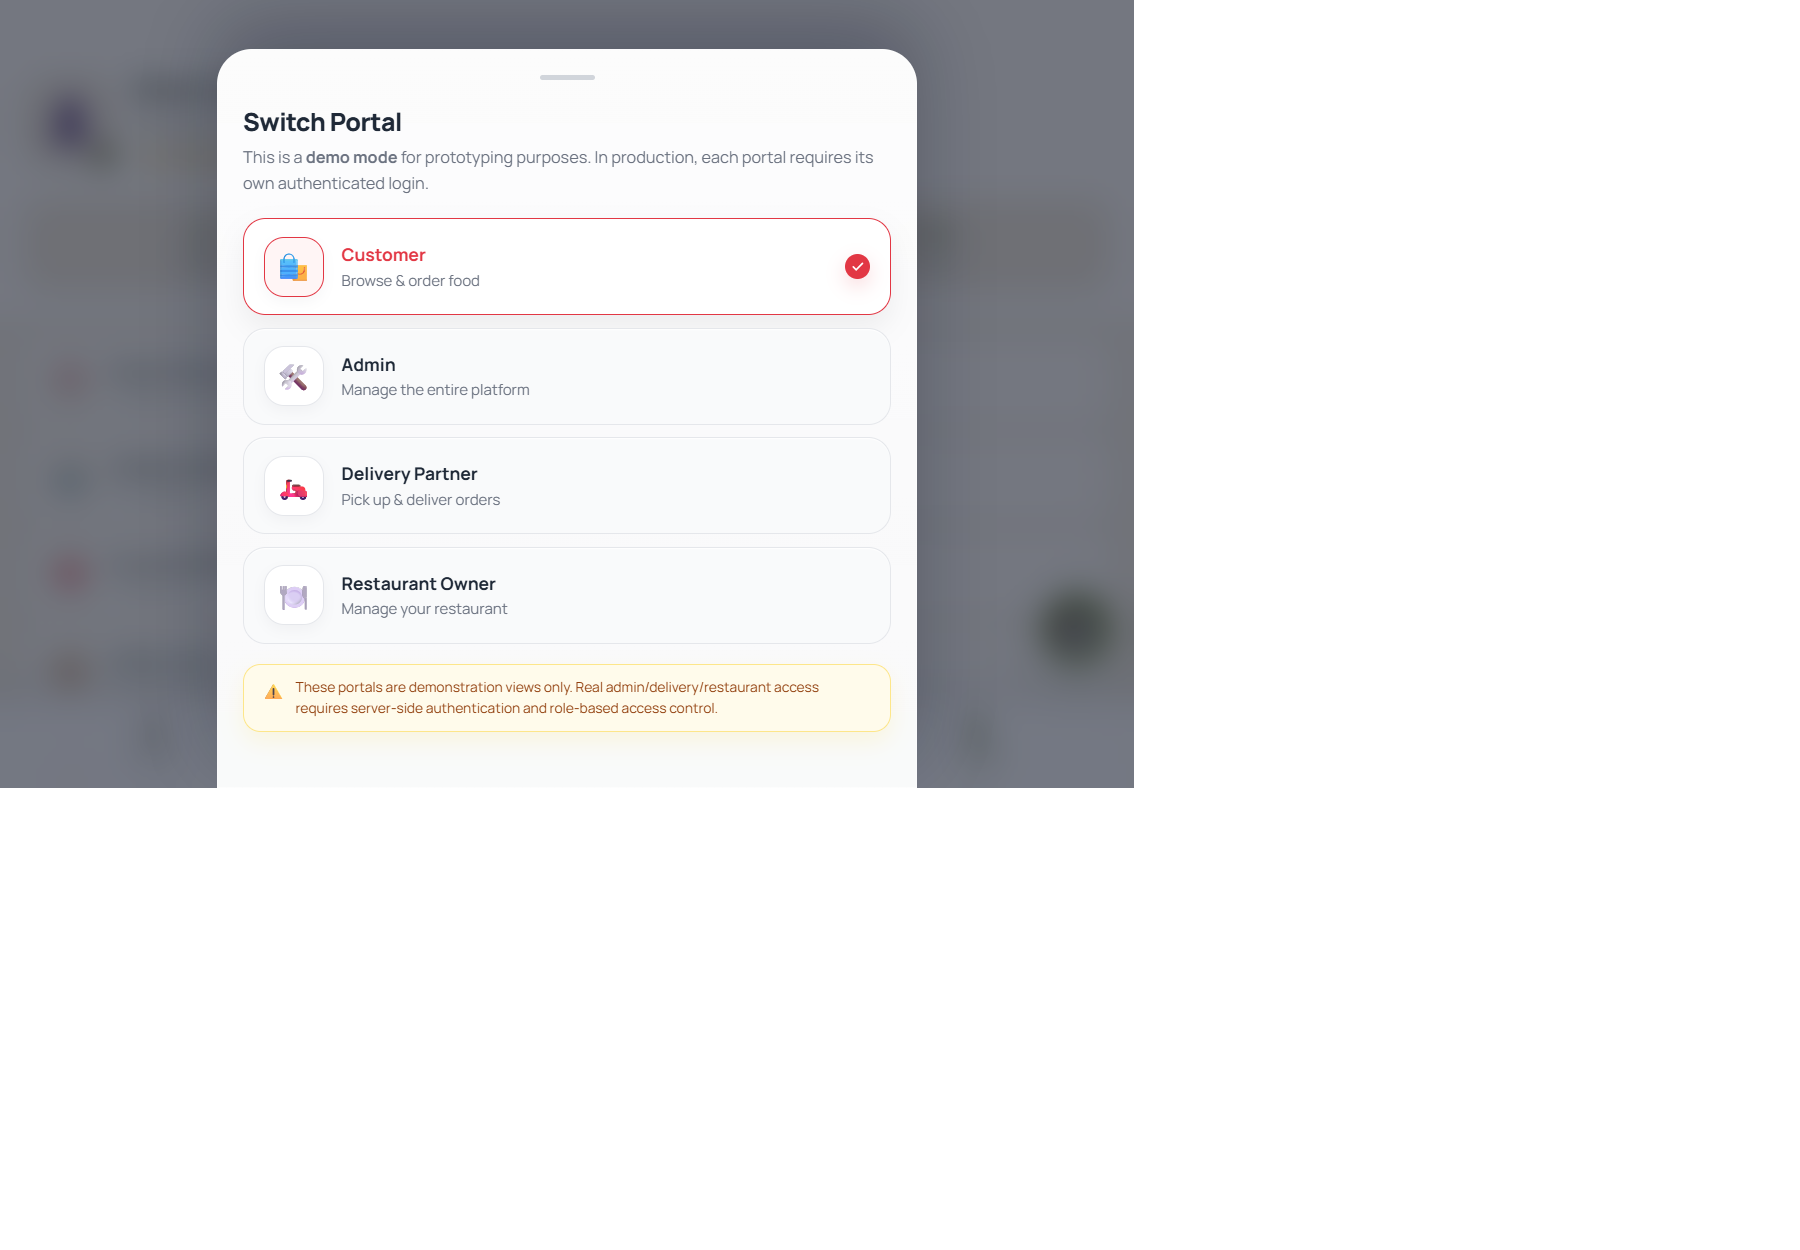
\includegraphics[
        width=0.9\textwidth,
        height=0.4\textheight,
        keepaspectratio
    ]{Chapters/role_selection.png}

    \caption{Portal switcher, explicitly identified in the application as demo functionality}
    \label{fig:portal_switcher}
\end{figure}
